\begin{center}
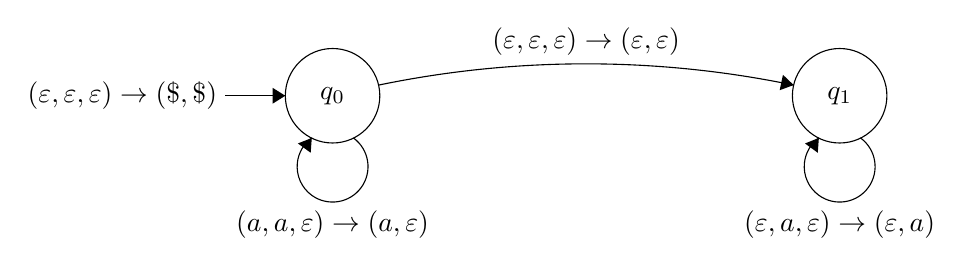
\begin{tikzpicture}[scale=0.2]
\tikzstyle{every node}+=[inner sep=0pt]
\draw [black] (24.1,-25.7) circle (3);
\draw (24.1,-25.7) node {$q_0$};
\draw [black] (56.3,-25.7) circle (3);
\draw (56.3,-25.7) node {$q_1$};
\draw [black] (17.3,-25.7) -- (21.1,-25.7);
\draw (16.8,-25.7) node [left] {$(\varepsilon,\varepsilon,\varepsilon)\rightarrow(\$,\$)$};
\fill [black] (21.1,-25.7) -- (20.3,-25.2) -- (20.3,-26.2);
\draw [black] (25.423,-28.38) arc (54:-234:2.25);
\draw (24.1,-32.95) node [below] {$(a,a,\varepsilon)\rightarrow(a,\varepsilon)$};
\fill [black] (22.78,-28.38) -- (21.9,-28.73) -- (22.71,-29.32);
\draw [black] (27.022,-25.024) arc (101.7088:78.2912:64.934);
\fill [black] (53.38,-25.02) -- (52.7,-24.37) -- (52.49,-25.35);
\draw (40.2,-23.17) node [above] {$(\varepsilon,\varepsilon,\varepsilon)\rightarrow(\varepsilon,\varepsilon)$};
\draw [black] (57.623,-28.38) arc (54:-234:2.25);
\draw (56.3,-32.95) node [below] {$(\varepsilon,a,\varepsilon)\rightarrow(\varepsilon,a)$};
\fill [black] (54.98,-28.38) -- (54.1,-28.73) -- (54.91,-29.32);
\end{tikzpicture}
\end{center}
